%  !TeX root = ../main.tex

\chapter{Symmetry}

\paragraph{What is symmetry?}

\begin{enumext}
  \item Leibniz: Symmetry is \emph{indiscernability of
    \sout{differences} changes \textrightarrow transformations}.
  \item Physical: invariance (under) transformations.
\end{enumext}

\subparagraph{Action part.}

V is the Hilbert space, and we have a map $V \mapsto V$, which is
the operator. The map is invertible.
Transformation stands for something like $X \mapsto \Omega(X)$,
i.e., map something to something else, but ``something else''
is in the same space, such as mapping a vector to a vector.
For example,
\[
\begin{cases*}
  \ket|\psi>  \mapsto \hat\Omega \ket|\psi>,& Transformation of state\\
  \hat O      \mapsto \hat\Omega \hat O \hat\Omega^{-1},
& Transformation of Operator\\
  \phi(x)     \mapsto (\Omega \phi)(x),     & Path Integral
\end{cases*}
\]

\subparagraph{Invariance part.}

When $X \sim Y$, i.e., $X$ is equivalent to $Y$, then it calles the
invariance.
After the map, we get something equivalent to $X$: $\Omega(x) \sim X$.
The invariance in the context can be, for example
\[
  \text{equations / constraints}\ \Omega(x) \sim X \longrightarrow
  \begin{cases*}
    \Omega \ket|\psi> = \ket|\psi> \upe^{\iu\varphi} &
    Transformation of state\\
    \hat\Omega \hat H \hat\Omega^{-1} = \hat H       &
    Transformation of Operator\\
    \mathcal S[\phi] = \mathcal S[\Omega\phi]        &
    Path Integral
  \end{cases*}
\]
To symmetry, $\Omega(x) \sim X$ is just equations/constraints:
Each equation is a kind of constraint on the object.

\vskip1ex \hrule
\subparagraph{Symmary}

For symmetry constraints, what constraints do is a limited possibility:
it is simplicity, or what understandability comes from.
How this happens is related to \emph{Symmetry \& Group Theory.}

The group is a set: we consider a set of transformation $\Omega_i$
\[
  G = \{\Omega_i\}, \qq{and the operation} \Omega_1 \circ \Omega_2
\]
The operation says that $\circ:\ G \times G \to G$.
Concerning the basic properties of Group
\begin{enumext}
  \item Closure: If $\Omega_{1,2}(X) \sim X$, then the combination
  $\Omega_1(\Omega_2(X)) \sim \Omega_i(X) \sim X$ is also in this set.
  \item Identity: Also okay, to do nothing.
  \item Inverse: We can have $\Omega(X) \sim X$ then do the inverse
  $\Omega^{-1}$ on both side
  \[
    X \sim \Omega^{-1}(X)
  \]
  By equivalent, this is so-called the inflective.
  \item Associativity: Such as by Hamiltonian, etc.
\end{enumext}
Referring to the Group theory, we shall talk about the

\section{Group Representation Theory}

\begin{enumext}
  \item Group: Introduce the space; elementary ``particles''
  \item Representation: We can ``lable'' (name) all the representations
  \begin{enumext}
    \item Different labels, which is closely related to conserved quantities
    (quantum numbers);
    \item Dimension: closely related to degeneracy.
  \end{enumext}
\end{enumext}

\subsection{Translation}

A trivial example is just to move the entire function $\phi(x)$ towards one
direction by $a$, we get
\[
  \phi(x) \mapsto \phi(x - a) \equiv \tilde \phi(x)
\]
where $x \in \mathbb R$. And we can define the translation operator $\hat T_a$
\[
  \phi(x - a) = \tilde \phi(x) = (\hat T_a\phi)(x)
\]
where $\phi(x)$ is the wavefunction, and we can get the new state
\[
  \phi(x) = \braket<x|\phi> \mapsto \phi(x - a) = \braket<x|\hat T_a\phi>
\]
Try to write it in the way of expansion
\[
  \hat T_a\ket|\phi> = \int \d x \ket|x> \braket<x|\hat T_a\phi>
= \int \d x \ket|x> \phi(x - a)
\xlongequal{\tilde x = x - a} \int \d x \ket|x - a> \phi(x)
\]
So, this transformation operator is a linear operator.
Insert the identity
\[
  \ket|\phi> = \int \d x \ket|x> \braket<x|\phi>, \qq{then,}
  \hat T_a\ket|\phi> = \int \d x \hat T_a \ket|x> \phi(x)
\]
In short, we have
\[
  \hat T_a\ket|x> = \ket|x + a>
\]
If $\ket|x>$ refers to a delta function $\delta(x)$, then the transformation
just move it to $\delta(x + a)$.
To write $T_a$ in basis
\[
  \hat T_a = \int \d x \ketbra|x + a><x|
\]
\paragraph{Quiz.}
Try to compute $\hat T_a \hat T_b$.
\[
  \hat T_a \hat T_b = \hat T_{a+b=b_a} = \hat T_b \hat T_a
\]

\subsection{Reflection}

\[
  \phi(x) \mapsto \phi(2a - x)
\]
We call the operation $\rho_a$.
The same logic.
\[
  \hat\rho_a\ket|\phi> = \int \d x \ket|x> \braket<x|\hat\rho_a\phi>
= \int \d x \ket|x> \phi(2a - x) = \int \d x \ket|2a - x> \phi(x)
\]
\textbf{Remember no minus sign here: the integration range also reversed.}
So, we obtain
\[
  \hat \rho_a\ket|x> = \ket|2a - x>
\]
\paragraph{Quiz}
Compute $\hat \rho_a \hat \rho_b$.
\[
  \hat\rho_a \hat\rho_b = \hat T_{2a - ab}
\]

\paragraph{Quiz}
Compute $\hat \rho_a \hat \rho_b \hat \rho_c$.
\[
  \hat\rho_a \hat\rho_b \hat\rho_c = \hat \rho_{a-b+c}
\]
There are some identities
\begin{align}
  \hat\rho_a^2 & = \identity,\\
  \hat\rho_a \hat\rho_b & \neq \hat\rho_b \hat\rho_a, \qq{where $a \neq b$}
\end{align}

\paragraph{Quiz}
Prove if $\hat T_a \hat \rho_b \overset?= \hat\rho_b\hat T_a$.
\[
  \hat T_a = \rho_{a/2} \rho_0
\]
So, $\hat T_a \hat \rho_b = \rho_{a/2+b}$, and
$\hat\rho_b\hat T_a = \rho_{b-a/2}$. They are not equal.

\subsection{Invariance}

\paragraph{With translation}

If we compose
\[
  \hat T_a \ket|\phi> = \upe^{\iu\phi} \ket|\phi>
\]
then, the wavefunction $\braket<x|\phi>$ must be periodic.
\emph{The formula above becomes the eigen equation.}
We can consider it as a complex plane wave $\upe^{\iu kx}$, i.e.,
a series loop, perpendicular to $x$.
Then, the wavelength is proportional to the period.

\paragraph{With Reflection}

Consider the eigen value equation
\[
  \hat\rho_a \ket|\psi> = \upe^{\iu\varphi} \ket|\psi>
\]
and we have the identity $\hat\rho_a^2 = \identity$,
then, the eigenvalue $\lambda^2 = 1$, $\lambda = \pm 1$.

Let $a \in \mathbb R$, which is continuous,
then we can have $\hat T_a \xlongrightarrow{a\to0} \identity$.

Consider a seires of atoms and the mirror planes,
\begin{center}
  \begin{tikzpicture}
    \draw (0,0) -- (7,0);
    \foreach \a in {1,2,...,6}
      {
        \draw (\a,0) circle (.1);
        \draw [dashed] ({\a + .5},1) --++ (0,-2);
      }
    \draw [->] (3.5,-1) --++ (1,0) node [below, midway] {$\hat T_a$};
  \end{tikzpicture}
\end{center}
the two mirror planes is related to $\hat T_a$.
It is not possible to have a $a$ to make $\hat \rho_a \to \identity$.

With the two examples above, we can generalize
\paragraph{General Transformation $\hat\Omega$}

The operator $\hat \Omega$ is unitary, and sometimes it can be anti-unitary,
and it is time-reversal.
The operator acts on states (vectors in Hilbert Space)
\[
  \ket|\psi> \mapsto \hat\Omega\ket|\psi>
= \sum_\alpha \hat\Omega \ket|\alpha> \psi(\alpha)
\]
always induce an action $\hat \Omega$ on operators
\[
  \hat O = \sum_{\alpha\beta} O_{\alpha\beta} \ketbra|\alpha><\beta|
\]
Then, the action $\hat \Omega$ on operators always induce
\[
  \hat O \mapsto
  \sum_{\alpha\beta} O_{\alpha\beta} \ketbra|\Omega\alpha><\Omega\beta|
\]
It is trivial that $\ket|\Omega\alpha> = \Omega\ket|\alpha>$,
but $\bra<\Omega\beta| = \bra<\beta|\Omega^{-1}$.
$\Omega$ is unitary, means that whatever $v$,
\[
  \braket<\Omega u|v> = \braket<\Omega^{-1}\Omega u|\Omega^{-1}v>
= \braket<u|\Omega^{-1}|v>.
\]
So, we have
\[
  \sum_{\alpha\beta} O_{\alpha\beta} \ketbra|\Omega\alpha><\Omega\beta|
= \hat\Omega \hat O\hat\Omega^{-1}
\]

\section{Continuous symmetry and conservation laws}

\subsection{Continuous symmetry}

\underline{Continuous is connected to $\identity$}
\[\begin{array}{ccc}
  \hat\Omega_\theta &
  \xlongleftrightarrow[\hat\Omega_\epsilon = \identity-\iu\epsilon\hat g]
    {\text{infinitesimal}} & \hat g\\
  \downarrow &  & \downarrow\\
  \text{Unitary} & & \text{Hermition}
\end{array}\]
We can give the
\begin{theorem}[Stone's theorem]
  $\forall u$, $v$, the inner product
  \[
    \braket<u|v> = \braket<\Omega_\epsilon u|\Omega_\epsilon v>
  \]
  \begin{proof}
    \[
      \cancel{\braket<u|v>}
    = \cancel{\braket<u|v>}
    + \iu\epsilon(\braket<\hat gu|v> - \braket<u|\hat gv>)
    \]
    then, we obtain
    \[
      \braket<\hat gu|v> = \braket<u|\hat gv>
    \]
    and the adjoint
    \[
      \braket<\hat Ou|v> = \braket<u|\hat O'v>
    \]
    If this is illegal $\forall u$, $v$, then we have
    \[
      \hat O' = \hat O^\dagger = \hat O
    \]
  \end{proof}
\end{theorem}
So, the generator $\hat g$ in this sense can be expressed as
\[
  \hat g = \iu\frac{\hat\Omega_\epsilon - \identity}{\epsilon}
            \bigg|_{\epsilon\to0}
= \iu \odv{\hat\Omega_\theta}\theta \bigg|_{\theta=0}
\]
\paragraph{With translation}

Given the definition
\[
  \hat T_a\ket|x> = \ket|x + a>
\]
then, consider $\hat T_a \hat x \hat T_a^{-1}$.
SInce $\hat x = \int \d x \ketbra|x> x <x|$
\[
  \hat T_a \hat x \hat T_a^{-1}
= \int \d x \ketbra|x - a> x <x + a| = \hat x - a
\]
Assume $a \to \epsilon$, then, we have
\[
  \hat T_\epsilon \hat x \hat T_\epsilon^{-1} = \hat x - \epsilon
\]
Substitute $\hat T_\epsilon = \identity - \iu\epsilon\hat g_T$, we have
\[
  (\identity - \iu\epsilon \hat g_T) \hat x (\identity + \iu\epsilon \hat g_1)
- \iu\epsilon(\hat g_T\hat x - \hat x \hat g_T) = -\epsilon
\]
which means
\[
  [\hat x, \hat g_T] = \iu, \qq{obviously,} \hat g_T = \hat k
\]

\paragraph{With rotation}

Consider the action (in 3D)
\[
  \hat R_{(\bm e_a, \epsilon)} \ket|\bm r> = \ket|?>
\]
Firstly, $\delta\bm r = \epsilon \bm e_a \times \bm r$, then,
\[
  \hat R_{(\bm e_a, \epsilon)} \ket|\bm r>
= \ket|\bm r + \epsilon \hat e_a \times \bm r>
\]
So, we have
\[
  \hat R_{(\bm e_a,\epsilon)} \hat{\bm r} \hat R_{(\bm e_a,\epsilon)}^{-1}
= \hat{\bm r} + \epsilon \bm e_a \times \hat{\bm r}
\]
The generator
$\hat R_{(\bm e_a,\epsilon)} = \identity - \iu\epsilon \hat g_{\bm a}$,
we can simply replace $\epsilon$ with the whole term
\[
  [\hat{\bm r}, \hat g_{\bm e_a}] = \iu\bm e_a \times \hat{\bm r}
\]
The key difference is that the equation is the vector equation, for the scalar,
\[
  [\hat x, \hat g_{\bm e_a}] = \iu(\bm e_a \times \hat{\bm r})_x
\]
To expand it,
\[
  [\hat x, \hat g_{\bm e_a}] = \iu [(e_a)_y\hat z - (e_a)_z \hat y]
\]
Similarly, for $\hat y$ and $\hat z$, the single equation corresponds to 3
sub-equations in total.
Eventually, we will find
\[
  \hat g_{\bm e_a} = \bm e_a \cdot(\hat{\bm r} \times \hat{\bm k})
= \bm e_a \cdot \hat{\bm L}
\]
where $\hat{\bm L} \equiv \hat{\bm r} \times \hat{\bm k}$.
If the rotation is actually the symmetry, then, the projection $\bm e_a$ can be
removed.

If $a$ is no more infinitesimal, i.e.,
to the exponential $U(t) = \upe^{-\iu\hat Ht}$,
we can divide $a$ into $n$-steps, then take the multiplication into power $N$ of
small steps of translations
\[
  \hat T_a = \identity - \iu\epsilon \hat g_T \Rightarrow
  \hat T_a = (\hat T_{a/N}) \xlongequal{N\to\infty}
  \ab(1- \iu\frac aN \hat g_T)^N = \upe^{-\iu a\cancelto{k}{\hat g_T}}
\]
Similarly for the rotation, we have
\[
  \hat R_{(\bm e_a,\epsilon)} = \identity - \iu\epsilon \hat g_{\bm a}
  \Rightarrow
  \hat R_{(\bm e_a,\epsilon)} = \upe^{-\iu\theta \bm e_a \cdot \hat{\bm L}}
= \upe^{-\iu \bm\theta \cdot \hat{\bm L}}
\]
Usually, we say $\bm e_a$ is fixed, then we have only one parameter $\theta$.
Now, we can rewrite this trivially
\[
  \hat R_{\bm\theta} = \upe^{-\iu\bm\theta\hat{\bm L}}
\]
It means we have 3 free parameters, which allows us to do the exponential
mapping.
Functions themselves make the Hilbert space: $\{f(\bm r)\}$
\[
  f(\bm r) = (\hat Rf)(\bm r)
\]

\paragraph{TL;DR}

$\hat g_\Omega$ is the transformation generator of the rotation
symmetry $\hat\Omega_\epsilon$
\begin{equation}
  \hat \Omega_\epsilon = \identity - \iu\epsilon \hat g_\Omega
\end{equation}
The equation of the rotation operator
\begin{equation}
  \hat R_
    {(\underset{\text{axis}}{\bm e_a}, \underset{\text{angle}}{\vphantom{\bm e_a}\epsilon})} =
  \ket|\bm r + \epsilon \bm e_a \times \bm r>.
\end{equation}
It change the eigenstate from $\ket|\bm r>$
to $\ket|\bm r + \epsilon \bm e_a \times \bm r>$.
The equation of the generator of the operator is
\begin{equation}
  [\hat{\bm r}, \hat g_{\bm e_a}] = \iu \bm e_a \times \bm r.
\end{equation}
Consider each component of the vector $\hat{\bm r}$
($\bm r = (r_1, r_2, r_3) = (x, y, z)$)
\[
  [\hat r_i, \hat g_{\bm e_a}] = \iu [(e_a)_2\hat r_3 - (e_a)_3\hat r_2]
= \iu [(e_a)_2\hat r_3 - (e_a)_3\hat r_2] \hat k_1 + (312) + (123)
= (\bm e_a \times \hat{\bm r}) \times \hat{\bm k} = \bm e_a \cdot \hat{\bm L}
\]
where $\hat g_{e_a} = \bm e_a \cdot \hat{\bm r}$, $\hat L \equiv \hat{\bm r} \times \hat{\bm k}$.

Then, we take the Infinitesimal (single-parameter)
\[
  \hat R_{(\bm e_a, \theta)} = \hat R_{(\bm e_i, \frac\theta N)}^N
= \ab(1- \iu\frac aN \hat g_T)^N = \upe^{-\iu \theta \bm e_a \cdot \hat{\bm L}}
\xlongequal{\theta \bm e_a \equiv \bm\theta} \upe^{-\iu\theta \cdot \bm{\hat L} = \sum_{j = 1,2,3} \theta_j \hat L_j}
\]

\paragraph{Translation Symmetry}

The operator $\hat T_{\bm a} \ket|\bm r> = \ket|\bm r + \bm a>$.
When act on a state $\ket|\psi>$ in the basis of real state
\begin{equation}
  \braket<\bm r|(\hat T_a|\psi>) = \braket<\bm r - \bm a|\psi>
= \psi(\bm r - \bm a)
\end{equation}
where consider it is unitary transformation operator
\[
  \bra<\bm r|\hat T_a = \bra<\hat T_{-a}| \bm r = \bra<\bm r - \bm a|
\]
and $\psi(\bm r) = \braket<\bm r|\psi>$. We can have the map
\begin{equation}
  \hat T_{\bm a}:\ \psi(\bm r) \longmapsto (\hat T_a\psi)(\bm r)
  \equiv \psi(\bm r - \bm a)
\end{equation}
Similarly, for the rotation
\begin{equation}
  \hat R_{\bm\theta = \bm e_a\theta} \ket|\bm r> = \ket|R_{\bm\theta} \bm r>
\end{equation}
i.e., in the vector form
\[
  \begin{pmatrix}
    x\\y\\z
  \end{pmatrix} \to
  \begin{pmatrix}
    x'\\y'\\z'
  \end{pmatrix} = \hat R_{\bm g}
  \begin{pmatrix}
    x\\y\\z
  \end{pmatrix}
\]
where $\bm r = (x, y, z)\tran$ $\bm r' = (x',y',z')\tran$.
Since the norm of the vectors are conserved, i.e.,
\begin{equation}
  {\bm r'}\tran\bm r' = \bm r\tran\bm r
= \bm r\tran\hat R_{\bm\theta}\tran\hat R_{\bm\theta}\tran \bm r
\end{equation}
Then, we can derive
\begin{equation}
  \hat R_{\bm\theta} = \upe^{\bm\theta \cdot \hat{\bm L}}
\end{equation}
from which
\[
  \begin{cases}
    \hat R_{\bm\theta}\tran \hat R_{\bm\theta} = \identity,\\
    \det(\hat R_{\bm\theta}) = +1.
  \end{cases}
\]
We can have the anti-symmetric real matrix $\hat{\bm L}$
\begin{equation}
  L_i\tran = -L_i
\end{equation}
where can be expanded as
\begin{equation}
  \begin{pmatrix}
    0 & a & b\\
    -a & 0 & c\\
    -b & -c & 0
  \end{pmatrix} = a
  \begin{pmatrix}
    & 1\\-1\\ & & 0
  \end{pmatrix} + b
  \begin{pmatrix}
    & & 1\\ & 0\\ -1
  \end{pmatrix} + c
  \begin{pmatrix}
    0\\ & & 1\\ & -1
  \end{pmatrix}
  = a \hat L_3 + b \hat L_2 + c \hat L_1
\end{equation}
where thet label $1$, $2$, $3$ means that the naught $0$ on the third / second /
first row.
We can have the expooniential form, e.g.,
\[
  \upe^{a\hat L_3} =
  \begin{pmatrix}
    \cos a & -\sin a & 0\\
    \sin a & \cos a & 0\\
    0 & 0 & 1
  \end{pmatrix}
\]
where we use the identity
\[
  \pdiagmat[empty = {}]{A,0}^n = \pdiagmat[empty = {}]{A^a,0}
\]
Then, theeuqation for the opeartor becomes
\begin{equation}
  \braket<\bm r|\hat R_\theta|\psi> = \braket<\hat R_{-\bm\theta} \bm r|\psi>
\end{equation}
and we have the map
\begin{equation}
  \hat R_{\bm \theta}:\
  \psi(\bm r) \longmapsto (\hat R_{\bm\theta} \psi) (\bm r)
\equiv \psi(R_{-\bm\theta} \bm r)
\end{equation}
The transfromation in coordinate space induces the transformation in
Hilbert space. The generator
\[
  \hat{\bm g}_{\hat R_{\bm\theta}} = \hat{\bm L} = (\hat L_1, \hat L_2, \hat L_3)
\]
and the commutators
\begin{align}
  \hat T_{a_y} \hat T_{a_x} \ket|\bm r> & = \ket|\bm r + a_x\hat x + a_y \hat y>,\\
  \hat R_{\theta_y} \hat R_{\theta_x} \ket|\bm r> &
= \ket|\hat R_{\theta_y} \hat R_{\theta_x} \bm r>
\neq \ket|\hat R_{\theta_x} \hat R_{\theta_y} \bm r>
\end{align}

\paragraph{Quiz} Calculate $[\hat L_1, \hat L_2]$.

Back to the commutator
\[
  [\hat L_1, \hat L_2]
= [\hat y\hat k_z, \hat z\hat k_x] + [\hat z\hat k_y, \hat x\hat k_z]
= [\hat y\hat k_z, \hat z] \hat k_x + \hat x[\hat z\hat k_y, \hat k_z]
= \hat y[\hat k_z, \hat z]\hat k_x + \hat x[\hat z, \hat k_z]\hat k_y
= \iu(\hat x\hat k_y - \hat y\hat k_x) = \iu\hat L_3
\]
So, there are three equations.

\subsection{Conservation Laws}

\begin{remark}[BCH]
  The commutator
  \[
    [A, \cdot] (BC) \equiv [A, BC] = [A, B]C + B[A,C], \qq{and}
    \pdif A(BC) = (\pdif AB)C + B(\pdif A)C
  \]
  also for $BC \to BCD$.
  Consider the BCH identity
  \[
    \upe^AB\upe^{-A} = B + [A, B] + \frac1{2!}[A,B]_2 + \cdots + \frac1{n!}[A,  B]_n
  \]
  where $[A, B]_n = [A, [A, \cdots [A, B \underset n{]]]} \mapsto \pdif A^n B$
\end{remark}
The transformation
\[
  \hat\Omega_\theta \hat H \hat\Omega_\theta^{-1} \mathbf = \hat H
\]
where $\hat H$ is time-independent.
We take the infinitesimal $\theta \to \epsilon$,
$\hat\Omega_\theta = \identity - \iu\epsilon\hat g_\Omega$.
It is trivial that
\[
  [\hat g_\Omega, \hat H] = 0
\]
Take the time-evolution operator
\[
  \hat U(t, 0) = \upe^{-\iu t\hat H}, \quad
  \hat U(\epsilon, 0) = \identity - \iu \epsilon \hat H
\]
then, we have the sandwitch
\[
  \hat U(t, 0) \hat g_\Omega \hat U(t, 0)^{-1} = \hat g_\Omega
\]
The evolution
\[
  \braket<\psi(0)|\hat g_\Omega|\chi(0)>
= \braket<\psi(t)|\hat U(t,0)\hat g_\Omega\hat U(t,0)^{-1}|\chi(t)>
= \braket<\psi(t)|\underset{\text{conserved quality}}{\hat g_\Omega}|\chi(t)>
\]
Then, the Schr\"odinger equation
\[
  \odv*{\ket|\psi(t)>}t = -\iu\hat H(t) \ket|\psi(t)>
\]
and the time derivative
\[
  \odv*{\braket<\psi(0)|\hat g_\Omega|\chi(0)>}t
= \iu\braket<\psi(t)|[\hat H(t), \hat g_\Omega]|\chi(t)> = 0
\]
It vanishes because the symmetry.

\paragraph{Energy conservation}

We certainly have one trival contribution that goint to give us the commutator
between $\hat H(t)$ and $\hat (t)$
\[
  \odv*{\braket<\psi(0)|\hat g_\Omega|\chi(0)>}t
= \iu\braket<\psi(t)|[\hat H(t), \hat H(t)|\chi(t)]>
+ \braket<\psi(t)|\underset{= 0}{\odv*{\hat H(t)}t}|\chi(t)>
\]
We can have $\hat H(t) = t\hat H_0$.

\begin{theorem}[Noether's Theorem]
  We need to change out language
  to $\mathcal S[q(t)] \mapsto \mathcal S[(\Omega_\alpha q)(t)]$.
  The continuous transformation of ``Path''
  \[
    \Omega_\theta:\ q(t) \longmapsto (\Omega_\theta q)(t) \equiv q_\theta(t)
  \]
\end{theorem}
In the examples, we can generally write
\[
  f(\epsilon) = f(0) + \epsilon f'(0), \qq{where} f(t) = \odv{q_\theta}\theta
\]
$q$ is still a function of time. Then,
\[
  q_\epsilon = q(t) + \epsilon f(t)
\]
\begin{example}[Translation]
  \[
    q_\epsilon(t) = q(t) + \epsilon, \quad f(t) = 1
  \]
  \begin{center}
    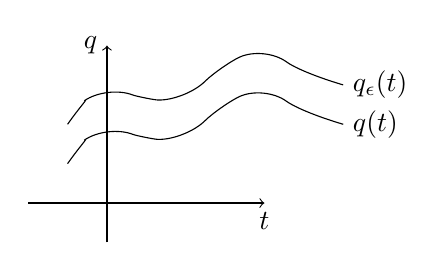
\begin{tikzpicture}[rounded corners = 10pt]
      \draw [->] (-1,0) -- (2,0) node [below] {$t$};
      \draw [->] (0,-.5) -- (0,2) node [left] {$q$};
      \draw (-.5,.5) to[bend left = 10] (0,1) to[bend right = 10] (1,.8)
        to[bend left = 10] (2,1.5) to[bend right = 10] (3,1)
        node [right] {$q(t)$};
      \draw [yshift = .5cm]
        (-.5,.5) to[bend left = 10] (0,1) to[bend right = 10]
        (1,.8)   to[bend left = 10] (2,1.5) to[bend right = 10] (3,1) node [right] {$q_\epsilon(t)$};
    \end{tikzpicture}
  \end{center}
\end{example}
\begin{example}[rotation]
  \[
    \bm q_\epsilon(t) = \bm q(t) + \epsilon \bm e_a \times q(t), \quad
    \bm f(t) = \bm e_a \times \bm q(t)
  \]
  The rotation of the world line.
  Figure: the world line rotate a angle between two time point real surface.
\end{example}
\begin{example}[time-translation]
  \[
    q_\epsilon(t) = q(t - \epsilon), \quad
    f(t) = -\dot q(t)
  \]
  \begin{center}
  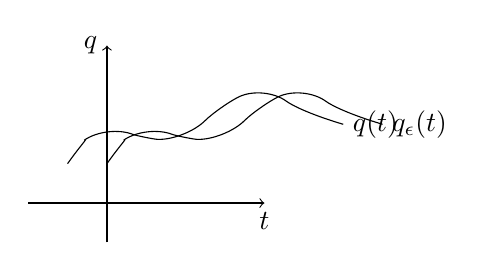
\begin{tikzpicture}[rounded corners = 10pt]
      \draw [->] (-1,0) -- (2,0) node [below] {$t$};
      \draw [->] (0,-.5) -- (0,2) node [left] {$q$};
      \draw (-.5,.5) to[bend left = 10] (0,1) to[bend right = 10] (1,.8)
        to[bend left = 10] (2,1.5) to[bend right = 10] (3,1)
        node [right] {$q(t)$};
      \draw [xshift = .5cm]
        (-.5,.5) to[bend left = 10] (0,1) to[bend right = 10]
        (1,.8)   to[bend left = 10] (2,1.5) to[bend right = 10] (3,1) node [right] {$q_\epsilon(t)$};
  \end{tikzpicture}
  \end{center}
\end{example}
For $t$-independent $\Omega_\theta$, the functional derivative
\begin{align*}
  0 & = \odv{\mathcal S[\Omega_\theta q]}\theta \bigg|_{\theta=0}
    = \frac1\epsilon (\mathcal S[\Omega_\epsilon q] - \mathcal S[q])
      \bigg|_{\epsilon \to 0}
    = \int_{t_i}^{t_f} \d t
      \ab(\pdv{\mathcal L}q \pdv{q_\theta}\theta
    + \pdv{\mathcal L}{\dot q} \pdv{\dot q_\theta}\theta) \\
    & = \int_{t_i}^{t_f} \d t
        \underbrace{\ab(\pdv{\mathcal L}q - \odv*{\pdv{\mathcal L}{\dot q}}t) f}
        _\text{E-L Equation}
      + \ab(\pdv{\mathcal L}{\dot q}f)\bigg|_{t_i}^{t_f}
\end{align*}
where we integral on shell, and
\[
  \mathcal S[q_\theta(t)] = \int_{t_i}^{t_f} \d t
  \mathcal L(q_\theta(t), \dot q_\theta(t), t)
\]
Since the E-L equation, we have
\[
  \ab(\pdv{\mathcal L}{\dot q}f)\bigg|_{t_i}^{t_f} = 0
\]
But $t_i$ and $t_f$ are arbitrary, so we can derive that
\[
  \odv*{\pdv{\mathcal L}{\dot q}f}t = 0
\]
means that it is independent from time, we get the conserved quantity.

So, in the first example $p$ is conserved; In the second one,
\[
  \mathcal S[q_\theta(t)] = \int_{t_i}^{t_f} \d t
  \mathcal L(\bm q_\theta(t), \dot{\bm q}_\theta(t), t)
\]
and
\[
  \ab(\sum_i \pdv{\mathcal L}{\dot q_i}f)\bigg|_{t_i}^{t_f} = 0
\]
so, $\bm e_a \cdot L = \bm p \cdot(\bm e_a \times \bm q(t))$
in the second example.

In the time-translation,
\[
  \mathcal S[q_\epsilon(t)] = \int_{t_i+\epsilon}^{t_f+\epsilon} \d t
  \mathcal L(q_\epsilon(t-\epsilon), \dot q_\epsilon(t-\epsilon), t)
\xlongequal{\tilde t = t - \epsilon} \int_{t_i}^{t_f} \d \tilde t
  \mathcal L(q(\tilde t), \dot q(\tilde t), \tilde + \epsilon)
\]
The derivative
\[
  0 = \odv{\mathcal S[\Omega_\theta q]}\theta \bigg|_{\theta=0}
    = \frac1\epsilon(\mathcal S[\Omega_\epsilon q] - \mathcal S[q])
    = \int_{t_i}^{t_f} \d t \pdv{\mathcal L}t \Rightarrow \pdv{\mathcal L}t = 0
\]
To interrupt it, we consider the total derivative
\[
  \odv*{\mathcal L}t = \pdv*{\mathcal L}q \dot q
+ \pdv*{\mathcal L}t\ab(\odv*{\dot q}t) + \pdv*{\mathcal L}t
\]
The second term
\[
  \pdv*{\mathcal L}t\ab(\odv*{\dot q}t)
= \odv*[fun]{\pdv{\mathcal L}q \dot q}t
- \ab(\odv*{\pdv{\mathcal L}{\dot q}}t)\dot q
\]
Substitute it and rearrange
\[
  0 = \pdv{\mathcal L}t = \odv*{\underbrace{\ab(
    \mathcal L - \pdv{\mathcal L}{\dot q} \dot q)}_\text{Hamiltonian}}t
- \underbrace{\ab(\pdv{\mathcal L}q - \odv*{\pdv{\mathcal L}q}t)}_
  \text{E-L equation} \dot q
\]
Then, we have the on-shell
\[
  \odv*{\mathcal H}t = 0
\]
i.e., the energy is conserved.

\paragraph{From (good) quantum numbers to group irrepresentation}

The statement is if
\[
  [\hat A, \hat B] = 0, \Rightarrow \exists \text{basis} \{\ket|\lambda>\}
\]
The basis vector is the eigenvector of both $\hat A$ and $\hat B$
\[
  \hat A\ket|\lambda> = \lambda_A\ket|\lambda>, \qq{and}
  \hat B\ket|\lambda> = \lambda_B\ket|\lambda>.
\]
\begin{proof}
  Consider $\hat A$ and $\hat B$ are Hermition.
  Take the ground state
  \[
    \hat A\ket|\alpha> = \alpha\ket|\alpha>
  \]
  In the case of degeneracy,
  \[
    \hat A\ket|\alpha_i> = \alpha\ket|\alpha_i>, \quad
    i = 1,\ \ldots\,,~d_\alpha
  \]
  Then, consider
  \[
    \hat A(\hat B\ket|\alpha>) = \hat B\hat A\ket|\alpha>
  = \alpha(\hat B\ket|\alpha>)
  \]
  means that
  \[
    \begin{cases*}
      \hat B\ket|\alpha> = b^{(\alpha)}\ket|\alpha>, & no-degeneracy\\
      \hat B\ket|\alpha_i> = \sum_j \ket|\alpha_j> b_{ji}^{(\alpha)}, &
      degeneracy
    \end{cases*}
  \]
  where $b_{ji}^{(\alpha)} = \braket<\alpha_j|\hat B|\alpha_i>$.
  We can always diagonalize
  \[
    b^{(\alpha_i)} = V D V^{-1}, \quad b^{(\alpha_i)} V = VD
  \]
  $D$ being a diagonal matrix $D_{ml} = \beta_l^{(\alpha)} \delta_{ml}$.
  Then,
  \[
    \sum_i b_{ji}^{(\alpha)} V_{il} = \sum_m V_{jm} D_{ml}
  = V_{jl} \beta_l^{(\alpha)}
  \]
  By take one superposition of the orginal $\alpha$
  \[
    \ket|\tilde \alpha_l> = \sum_i \ket|\alpha_i> V_{il}
  \]
  It is easy to know
  \[
    \hat B\ket|\tilde\alpha_\lambda> = \sum_i \hat B\ket|\alpha_i> V_{il}
  = \sum_{ij} \ket|\alpha_j>b_{ji}^{(\alpha)} V_{il}
  = \ket|\tilde\alpha_l> \beta_l^{(\alpha)}
  \]
  Then, the site
  \[
    \{\ket|\tilde\alpha_l>\} = \{\ket|\lambda>\}
  \]
  if there is no degeneracy, then $\ket|\tilde\alpha> = \ket|\alpha>$.
\end{proof}

\section{Symmetry group representations, degeneracies,
         inversion and time reversal}

\section{Angular momentum, Lie algebra}

\section{Gauge}
